\documentclass[12pt]{article}
\usepackage{graphicx}
\usepackage{minted}
\usepackage{hyperref}
\usepackage{float}

\begin{document}
\begin{titlepage}
  \begin{center}
    \large{University of Puerto Rico\\
    Mayagüez Campus\\
    \vspace{\baselineskip}
    Department of Electrical and Computer Engineering}
  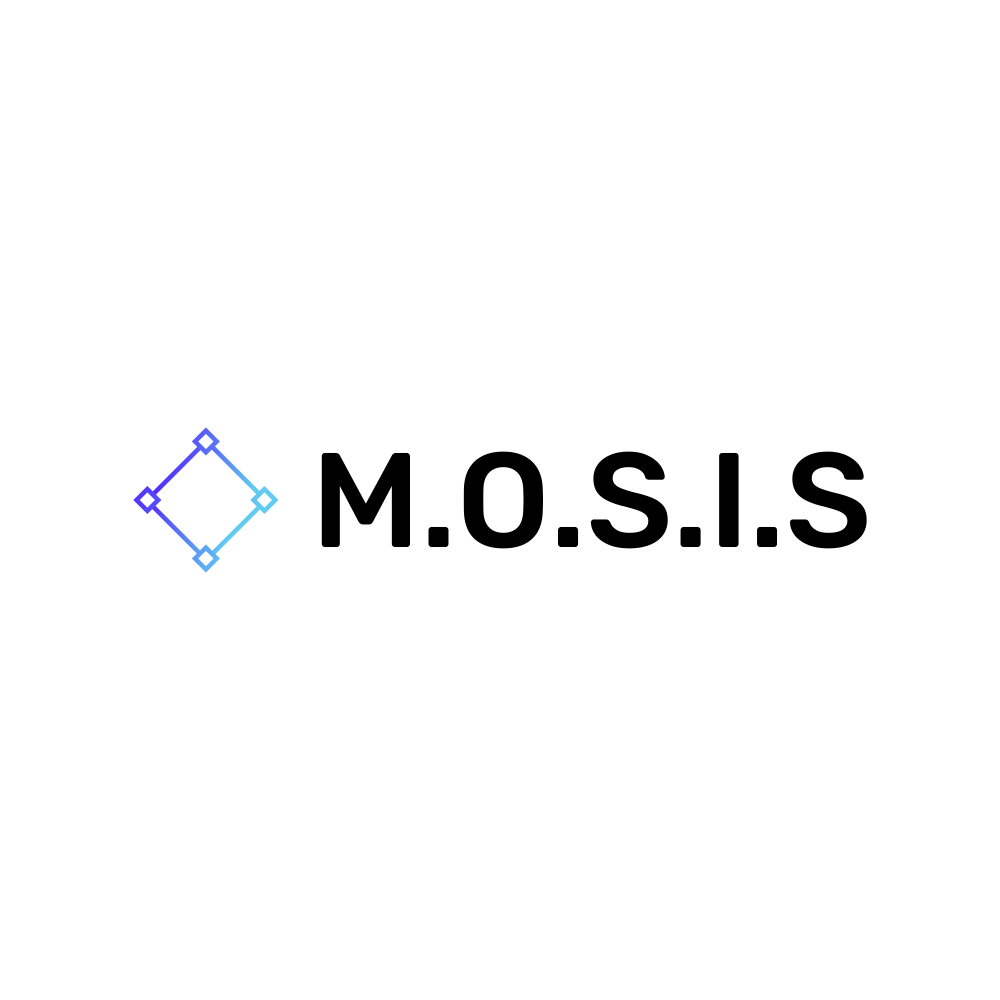
\includegraphics[scale=0.2]{../Title_Page/default.png}\\
    \Huge{\underline{M.O.S.I.S Host Software}\\}
    \Huge{\underline{User Guide}\\}
    \vspace{5cm}
    \large by\\
    Fabio J. Matos Nieves\\
    \normalsize
  \end{center}
\end{titlepage}

\tableofcontents
\newpage
\section{Installation}
\subsection{Windows}
\subsubsection{Installing Git}
In order get the host software we first have to install Git to clone the Host Software repository. We can download Git from \href{https://git-scm.com/download/win}{here}. You choose the ``64-bit Git for Windows Setup'' for the vast majority of cases. You should only opt for using ``32-bit Git for Windows Setup'' for very old computers. If prompted to where to download the file, select the ``Downloads'' folder. Once the Git installer has finished downloading, open the file explorer and go to the downloads folder as shown here:
After opening the downloads folder, double click on the on the Git installer and if a darkened screen appears asking for administrator privileges, press the yes button. Once the Git installer is open, follow these steps:
\begin{center}
	\begin{enumerate}
		\begin{figure}[H]
			\includegraphics[width=0.8\textwidth]{./Figures/OpenFileExplorer.png}
		\end{figure}
		\item Open the File Explorer from the taskbar at the bottom.
		      \begin{figure}[H]
			      \includegraphics[width=0.8\textwidth]{./Figures/OpenDownloadsFolder.png}
		      \end{figure}
		\item Click on the downloads folder on the left side bar.
		      \begin{figure}[H]
			      \includegraphics[width=0.8\textwidth]{./Figures/GitInstallerMenu1.png}
		      \end{figure}
		\item Double click on the Git installer and the installer should appear. Click on the next button.
		      \begin{figure}[H]
			      \includegraphics[width=0.8\textwidth]{./Figures/GitInstallerMenu2.png}
		      \end{figure}
		\item Click next.
		      \begin{figure}[H]
			      \includegraphics[width=0.8\textwidth]{./Figures/GitInstallerMenu3.png}
		      \end{figure}
		\item Click next.
		      \begin{figure}[H]
			      \includegraphics[width=0.8\textwidth]{./Figures/GitInstallerMenu4.png}
		      \end{figure}
		\item Click next.
		      \begin{figure}[H]
			      \includegraphics[width=0.8\textwidth]{./Figures/GitInstallerMenu5.png}
		      \end{figure}
		\item Click next.
		      \begin{figure}[H]
			      \includegraphics[width=0.8\textwidth]{./Figures/GitInstallerMenu6.png}
		      \end{figure}
		\item Click next.
		      \begin{figure}[H]
			      \includegraphics[width=0.8\textwidth]{./Figures/GitInstallerMenu7.png}
		      \end{figure}
		\item Click next.
		      \begin{figure}[H]
			      \includegraphics[width=0.8\textwidth]{./Figures/GitInstallerMenu8.png}
		      \end{figure}
		\item Click next.
		      \begin{figure}[H]
			      \includegraphics[width=0.8\textwidth]{./Figures/GitInstallerMenu10.png}
		      \end{figure}
		\item Click next.
		      \begin{figure}[H]
			      \includegraphics[width=0.8\textwidth]{./Figures/GitInstallerMenu11.png}
		      \end{figure}
		\item Click next.
		      \begin{figure}[H]
			      \includegraphics[width=0.8\textwidth]{./Figures/GitInstallerMenu12.png}
		      \end{figure}
		\item Click next.
		      \begin{figure}[H]
			      \includegraphics[width=0.8\textwidth]{./Figures/GitInstallerMenu13.png}
		      \end{figure}
		\item Click next.
		      \begin{figure}[H]
			      \includegraphics[width=0.8\textwidth]{./Figures/GitInstallerMenu14.png}
		      \end{figure}
		\item Click next.
		      \begin{figure}[H]
			      \includegraphics[width=0.8\textwidth]{./Figures/GitInstallerMenu15.png}
		      \end{figure}
		\item Click next.
		      \begin{figure}[H]
			      \includegraphics[width=0.8\textwidth]{./Figures/GitInstallerMenu16.png}
		      \end{figure}
		\item Click next.
		      \begin{figure}[H]
			      \includegraphics[width=0.8\textwidth]{./Figures/GitInstallerMenu17.png}
		      \end{figure}
		\item Wait for installation to complete.
		      \begin{figure}[H]
			      \includegraphics[width=0.8\textwidth]{./Figures/GitInstallerMenu18.png}
		      \end{figure}
		\item Click next.
	\end{enumerate}
\end{center}
Once Git is installed follow these steps to verify that Git installed correctly.
\begin{center}
	\begin{enumerate}
		\begin{figure}[H]
			\includegraphics[width=0.8\textwidth]{./Figures/SearchBar.png}
		\end{figure}
		\item Search Powershell in the search bar that is in the task bar at the bottom.
		      \begin{figure}[H]
			      \includegraphics[width=0.8\textwidth]{./Figures/PowershellSearchResult.png}
		      \end{figure}
		\item Click on the result that says ``Windows Powershell'' or where it says open. Do not click ``Run as administrator''.
		      \begin{figure}[H]
			      \includegraphics[width=0.8\textwidth]{./Figures/GitVersion.png}
		      \end{figure}
		\item To verify that Git installed correctly. Type the following command into Powershell and press enter.
		      \begin{minted}{ps1}
                        git -v
                      \end{minted}
		      It should reply with ``git version'' followed by version number.
	\end{enumerate}
\end{center}
\subsection{Downloading Host Software}
To download the host software itself, follow these steps:
\begin{center}
	\begin{enumerate}
		\begin{figure}[H]
			\includegraphics[width=0.8\textwidth]{./Figures/SearchBar.png}
		\end{figure}
		\item Search Powershell in the search bar that is in the task bar at the bottom.
		      \begin{figure}[H]
			      \includegraphics[width=0.8\textwidth]{./Figures/PowershellSearchResult.png}
		      \end{figure}
		\item Click on the result that says ``Windows Powershell'' or where it says open. Do not click ``Run as administrator''.
		\item Search Powershell in the search bar that is in the task bar at the bottom.
		      \begin{figure}[H]
			      \includegraphics[width=0.8\textwidth]{./Figures/GitCloneRepo.png}
		      \end{figure}
		\item Type the following command into the Powershell and press enter:
		      \begin{minted}[breaklines, breaksymbolleft=]{ps1}
git clone --depth 1 --no-single-branch https://github.com/fabiomatos999/M.O.S.I.S.git
                      \end{minted}
		\item Wait for the download to finish and then close Powershell.
	\end{enumerate}
\end{center}
\subsubsection{Installing wkhtmltopdf}
In order to get wkhktmktopdf, we can download it from \href{https://wkhtmltopdf.org/downloads.html}{here}. For the vast majority of cases, choose the ``Windows Installer 64-bit'' option and then the download should start. Once it has finished downloading, tn a similar fashion to installing Git, go to the Downloads folder in the File explorer and double click on the wkhtmltopdf installer. The following screen should appear and then proceed through the installation:
\subsubsection{Installing Ghostscript}
In order to get Ghostscript, we can download it down from \href{https://www.ghostscript.com/releases/gsdnld.html}{here}. For the vast majority of cases choose the ``Ghostscript for Windows (64 bit)'' option. Follow the instructions below:
\subsubsection{Installing Python}
In order to get Python, we can download it from \href{https://www.python.org/downloads/}{here}. Press the yellow download Python button on the page and the download should start. Again, find the Python installer in the Downloads folder. Double click on the executable file and follow the following steps carefully.
\subsubsection{Additional Setup}
In order to make the Host Software to run we need to make sure that Powershell scripts can be executed. First search for ``Windows Powershell'' in the search bar in the taskbar at the bottom of the screen but press the ``Run as administrator button'', if it prompts you to confirm running as administrator, press yes. Once Powershell is opened, type the following command into Powershell and press enter:
\begin{minted}{ps1}
  set-executionpolicy remotesigned
\end{minted}
It will then prompt you for additional input. Type ``Y'' and press enter. Then close Powershell.
\subsection{Linux}
\section{Start Host Software}
\subsection{Windows}
\subsection{Linux}
\section{Usage}
\subsection{Viewing All Captured Media}
\subsection{Viewing A Specific Captured Media}
\subsection{Search}
\subsubsection{ID}
\subsubsection{Shot Type}
\subsubsection{Illumination Type}
\subsubsection{Date}
\subsection{Study Profile Creation}
\subsection{Study Profile Upload}
\section{Backup Raspberry Pi Media}
\section{Backup Raspberry Pi SD Card}
\end{document}